% ---------------------------------------------------------------- 03-base-model.tex
\section{Results in the base model}\label{sec:base}

\subsection{The no-tax benchmark}\label{sec:notax}

Without taxes the all-equity firm U is worth $90/1.1 = 81.8$. A levered firm that promises creditors 80 pays them 80 in the strong state and the entire 60 in the weak state, where it defaults; shareholders receive 40 or 0. Debt is worth $70/1.1 = 63.6$ and equity $20/1.1 = 18.2$, which sum to 81.8. Because debt plus equity pays exactly what firm U pays in every state, the law of one price implies \eqref{eq:mm}: if the two packages were priced differently, buying the cheaper one and shorting the dearer one would lock in a profit today with zero payoff in both states, the trade of Lecture~1 (pp.~48, 60). Investors could reach the same result by homemade leverage, borrowing on personal account to turn U's shares into L's equity. Both routes assume no taxes, distress or trading costs (Lecture~1, p.~48).

\subsection{Corporate tax and the interest tax shield}\label{sec:tax}

With a 20\% tax the unlevered firm pays 24 or 12, so $\VU = 72/1.1 = 65.45$ and the present value of the government's claim is 16.36. A firm with $D = 40$ deducts interest of 4, so taxable income is 116 or 56 and tax is 23.2 or 11.2. Its investors receive 0.8 more in each state, and
\begin{equation}
  \VL - \VU = \frac{\tauc \rD D}{1 + r} = \frac{0.20 \times 0.10 \times 40}{1.10} = 0.73,
  \label{eq:shield}
\end{equation}
so that $\VL = 66.18$. The pie itself is unchanged, since $\VL$ plus the present value of taxes (15.64) still equals 81.8. Debt creates no cash flow; it transfers 0.73 from the government's claim to investors. Since \eqref{eq:shield} is proportional to $\tauc$, the gain vanishes at $\tauc = 0$ and the attribution condition is satisfied.

\subsection{Debt capacity and financial distress}\label{sec:capacity}

If each unit of debt added value, the firm would borrow without limit. It cannot, because the weak state's after-tax cash, $60 - 0.2(60 - 0.1D) = 48 + 0.02D$, must cover the promised repayment $1.1D$. The two are equal at
\begin{equation}
  \Dstar = \frac{(1 - \tauc) X_{\mathrm{w}}}{(1 + \rD) - \tauc \rD} = \frac{48}{1.08} = 44.4.
  \label{eq:dstar}
\end{equation}

Below $\Dstar$ every unit of debt adds shield (Table~\ref{tab:twostate}). At $D = 45$ the weak state defaults and loses 20\% of its 48.9 of cash (9.78), and $\VL - \VU$ falls from $+0.80$ to $-3.63$ (Figure~\ref{fig:value}a).

\begin{table}[htbp]\centering\footnotesize
\caption{Debt and firm value in the two-state model ($\tauc = 20\%$, $c = 20\%$)}\label{tab:twostate}
\begin{tabularx}{\linewidth}{@{}l*{4}{C}@{}}
\toprule
Debt $D$ & Weak-state after-tax cash & Promised repayment & Weak state defaults & $\VL - \VU$ \\
\midrule
40 & 48.80 & 44.00 & No  & $\phantom{-}0.73$  \\
44 & 48.88 & 48.40 & No  & $\phantom{-}0.80$  \\
45 & 48.90 & 49.50 & Yes & $-3.63$ \\
50 & 49.00 & 55.00 & Yes & $-3.55$ \\
\bottomrule
\end{tabularx}
\end{table}

\begin{figure}[htbp]\centering
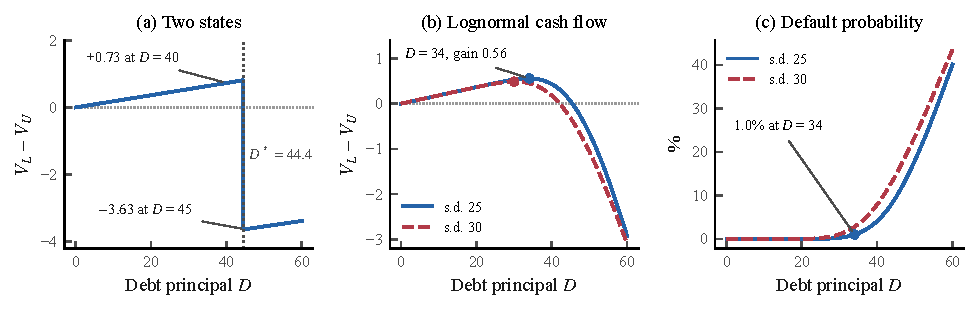
\includegraphics[width=\linewidth]{fig1_value}
\caption{Value of debt financing. (a) Two-state model: the gain rises to 0.81 at $\Dstar = 44.4$ and then collapses. (b) Lognormal cash flow with mean 90 and standard deviation 25 (200,000 draws), all other assumptions unchanged: the value function has an interior optimum near $D = 34$. (c) Default probability in the lognormal model. Dashed lines in (b) and (c) use a standard deviation of 30.}\label{fig:value}
\end{figure}

\textit{Where the money machine breaks down.} Rerun the trade of Lecture~1 (pp.~48, 60) with taxes: buy all of L's debt and equity and short U. At $D = 40$ it pays $+0.8$ in both states, so if the market priced L at $\VU = 65.45$ it would be a riskless money machine whose counterparty is the tax authority. Homemade leverage cannot copy it, because interest paid by an investor does not reduce the firm's tax bill; the law of one price survives and prices the shield, bidding $\VL$ up to $\VU + 0.8/1.1 = 66.18$, which is \eqref{eq:shield}. Borrowing more to collect more shield stops at $\Dstar = 44.4$: at $D = 45$ the weak state defaults and loses 9.78 of its 48.9 of cash, and the position pays $+0.90$ in the strong state but $-8.88$ in the weak one, worth $-3.63$. Without distress costs it would stay riskless beyond $\Dstar$ (Section~\ref{sec:sens}), so it is costly default, not the debt limit itself, that switches the machine off.

\subsection{Reading the result with the course toolkit}\label{sec:toolkit}

Three tools from the lectures read the base case directly. First, leverage moves risk between the slices while the pizza is unchanged (Lecture~2, p.~5). With $D = 40$, equity pays 52.8 or 4.8 and is worth 26.18; its payoff swings by 48, exactly as much as U's (96 or 48), but on a base of 26.18 instead of 65.45. Because debt and the one-year shield are riskless, all market risk sits in equity, so $\betaE = \betaU \times \VU/E = 2.5\betaU$ and, under CAPM, equity's risk premium is 2.5 times the unlevered firm's: a one-period Proposition II with taxes. Hamada's $1 + (1 - \tauc)D/E = 2.22$ is lower because it assumes a perpetual shield worth $\tauc D = 8$ rather than 0.73. Second, the WACC of Lecture~1 (p.~52) carries the same shield: $(26.18 \times 10\% + 40 \times 10\% \times 0.8)/66.18 = 8.79\%$, and discounting U's after-tax 72 at 8.79\% returns exactly $\VL = 66.18$. Third, the debt limit is a stress test in the sense of Lecture~5 (p.~23): \eqref{eq:dstar} asks whether creditors are paid in the weak state and needs no probability. The lognormal optimum has a VaR reading: at $D = 34$ the promise of 37.4 sits at the 1\% quantile of after-tax cash (37.4). The level is not a law; with $c = 5\%$ or 40\% the optimum accepts about 5\% or 0.4\% default risk. The tax rate sets the prize; the cost of failure, like expected shortfall beyond VaR (Lecture~5, pp.~19--20), sets how much tail risk the firm should accept.
